\documentclass[12pt,a4paper,oneside,final]{article}

\usepackage[utf8]{inputenc}
\usepackage{amsmath,amssymb,amsfonts}
\usepackage{bm}
\usepackage[hidelinks]{hyperref}

\usepackage[margin=1in]{geometry}
\usepackage{listings}
\usepackage{fancyhdr}
\usepackage{lastpage}
\usepackage{titlesec}

\usepackage{float}
\usepackage{graphicx}
\usepackage{caption}
\usepackage{subcaption}
\usepackage[section]{placeins}
\usepackage{color}

\pagestyle{fancy}
\addtolength{\headheight}{\baselineskip}
\setcounter{secnumdepth}{4}
\setcounter{tocdepth}{1}

\rhead{Vision and image processing \\ Assignment 4(5), 17/01-18}
\lhead{Therese Darum, zbl558; Cecilie Novak, bk662; \\ Christoffer Belhage, DZP300}
\cfoot{Page \thepage\ of \pageref{LastPage}}

\begin{document}

\section{Programming language and libraries used}
For this assignment \texttt{Matlab} and the handed out matlab functions \texttt{unbiased\_integrate.m} and \texttt{display\_detph.m}, which can be found at Absalon, have been used.

\section{Theory of photometric stereo}
Photometric stereo is a process of estimating a depth parameter for every pixel in an image that results in a depth map for the pixels in the image (also known as Monge patches).\\\\
As opposed to stereoscopic images, where images are taken at slightly different angles, photometric stereo uses several images taken from the exact same position, aiming at capturing the exact same scene as accurate as is possible, the only varying parameter being the placement of the (only) light source.\\\\
During the process, images where the light source is placed at different angles from image to image are taken and from these captured intensity values the depth map is inferred.\\\\
Assuming that the illuminated object has a rough surface (and is only illuminated by our single light source), the depth map can be inferred using Lambert's Law for diffuse reflection:
\begin{equation}
I(x,y) = \rho(x,y) n(x,y) \cdot S(x,y)
\end{equation}
where $I(x,y)$ is the image intensity value (i.e. the measured reflection of light from the object), $\rho(x,y)$ is the albedo value that defines the surface material's light absorbtion property and $n(x,y)$ is the normalized surface normal to the surface $S(x,y)$.\\\\
Since we only have a single light source, we can assume that there is no ambient light and we can model the intensities as
\begin{equation}
I(x,y) = \rho(x,y) n(x,y) \cdot S(x,y) = g(x,y) \cdot V
\end{equation}
where $g(x,y)$ describes the surface by its normal and albedo simultaneously, as suggested by Woodham, and $V$ is a vector giving the position and pointing direction of the light source. Since we know the intensity values $I(x,y)$ captured by the camera and the position and pointing direction of the light source $V$, we can solve the linear equations from the images, to calculate $g(x,y)$.\\\\
Once the $g(x,y)$ has been calculated, the albedo and the normalized surface normals can easily be recovered. Every vector $g(x,y)$ corresponds to the surface normalized normal vector $n(x,y)$ scaled by the albedo $\rho(x,y)$, so the albedo can be recovered by calculating $|g(x,y)|$ and the normalized normal vector as $\frac{g(x,y)}{|g(x,y)|}$.\\\\
Then, one can finally estimate the depth map (surface) by surface integration of the normalized normal vectors $n_1, n_2, n_3$ (for the setting using 3 images - if using more than 3 images, it will not necessarily be the normal vectors for image 1-3 that should be used).\\\\
There are a few considerations for this process to note: It is based on the assumption of an orthographic camera, however most cameras are perspective cameras. It is also assumed that the light source emits parallel light (the light source is placed FAR AWAY), but in reality, the emitted light is radially emitted, as it is unrealistic to be able to place the light source far enough away. As mentioned, we also assumed the surface of any object to be rough in order to leave out modelling of any specularities. In reality, not all objects have completely rough surfaces.

\section{Implementation}

To implement the photometric stereo, we have created the matrix for the albedo modulated normal field as $M = S^{-1} J$, where $S$ is the light sources and $J$ is the image intensities, in the areas where the binary mask indicates that we should solve for photometric stereo.\\\\
As the Beethoven image dataset is a synthetic example, we have used the "exact" inverse (as exact as it can become using computers, at least). This has been computed using the Matlab built-in function for calculation of inverse matrices. For the real example of the Buddha image dataset, we have used the pseudo-inverse (as we are not garanteed that the exact inverse exists when using real data). We have done this using the built-in Matlab function \texttt{pinv}.\\\\
The albedo and normal fields are then isolated from the $M$ matrix as described in the theory part (previous section).
Last, the depth map has been inferred by integration using the handed out Matlab function \texttt{unbiased\_integrate.m} and displayed using the handed out \texttt{display\_detph.m}.

\section{Results}
In figure \ref{fig:BeethovenDepth} we see the depth map we calculated for the Beethoven images from 3 angles. In figure \ref{fig:albedo}a we see the albedo within the mask. In the albedo image we observe highlights in the hair, around the collar and a few other places, indicating that here the material absorbs less light, meaning the material reflect a large part of the light. These are most likely due to the shape of the bust, we are trying to make a 3D model off. These particular areas of the bust are alway shadowed to a certain extent, thus creating the illusion that here the material absorbs more at the light. 
\begin{figure}[H]
	\centering
	\begin{subfigure}{.33\textwidth}
		\centering
		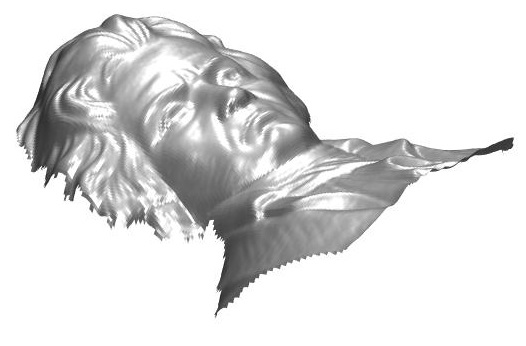
\includegraphics[width=5.5cm]{Beethoven1}
		\caption{Right}
	\end{subfigure}%
	\begin{subfigure}{.33\textwidth}
		\centering
		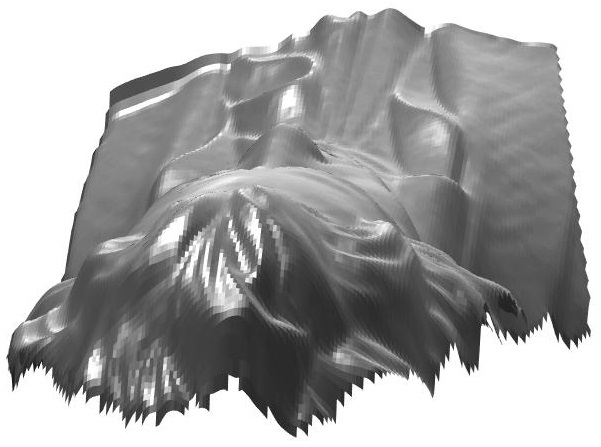
\includegraphics[width=5.5cm]{Beethoven2}
		\caption{Top}
	\end{subfigure}%
	\begin{subfigure}{.33\textwidth}
		\centering
		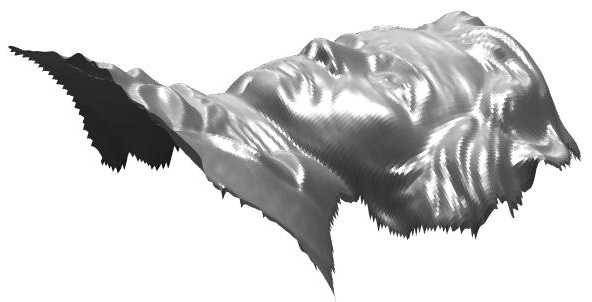
\includegraphics[width=5cm]{Beethoven3}
		\caption{Left}
	\end{subfigure}
	\caption{The Beethoven depth map from different view points}
	\label{fig:BeethovenDepth}
\end{figure}
With the clean synthetic image set of Beethoven, we get a very clean 3D model with a lot of details. The same cannot be said for the real Buddha image set. In figure \ref{fig:BuddahDepth} we see the calculated depth map of this set and in figure \ref{fig:albedo}b we see the corresponding albedo. The depth map is very flat, expect for the top part where the hair begins. We can see a hint of the nose and eyes. Part of the reason for the bad result is that the lights have been badly placed. The lights have been placed in such a way that large parts of the bust is completely in shadow in many of the images, making it difficult to extract depth information. Looking at the hair in figure \ref{fig:BuddahDepth} and the images we used for computation, we see that for all the images the hair is more evenly lit than the rest. This provide us with just enough shadow to compute accurate depth information. Another problem could also be the distance to the light source. As explained in the theory section, our computation assumes that the light beams are far away and thus parallel. If the light source is too close then it emits the light in a cone shape, meaning that the light source vector is different for different spots of the object, thus making our computation very inaccurate.
\\\\
A possible way to improve our results is to select the "good" lights, for example light from the right side, left side and front. This should provide us with enough shadows to compute a depth map, without introducing so much darkness that it becomes difficult to see depth differences. Alternatively we could try to select the 3 best images for each pixel, however this introduces a lot of complications, such as implementation difficulties, a need for intensity thresholding and problems with neighboring pixels not having the same light.
\begin{figure}[H]
	\centering
	\begin{subfigure}{.33\textwidth}
		\centering
		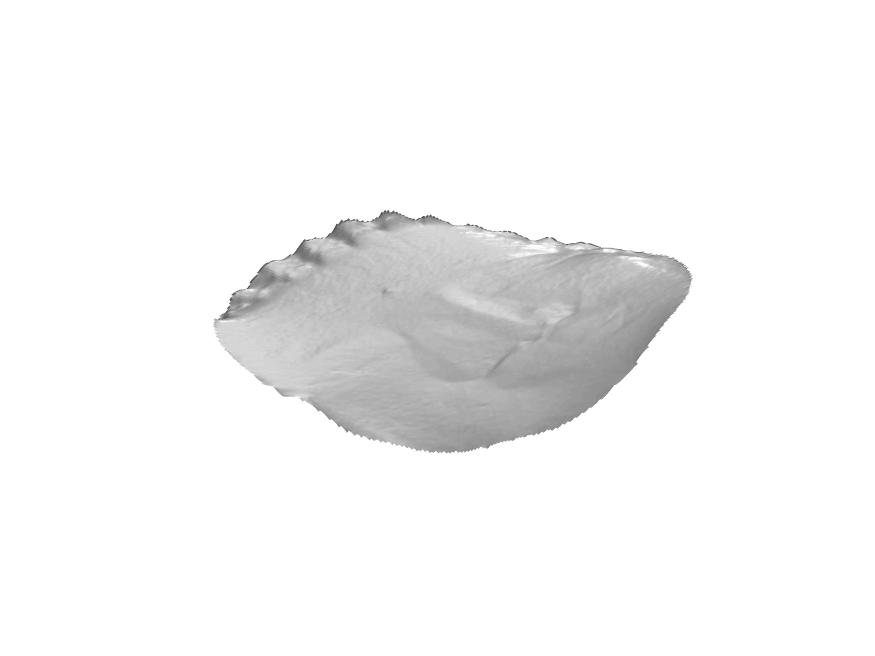
\includegraphics[width=5.5cm]{Buddha1}
		\caption{Right}
	\end{subfigure}%
	\begin{subfigure}{.33\textwidth}
		\centering
		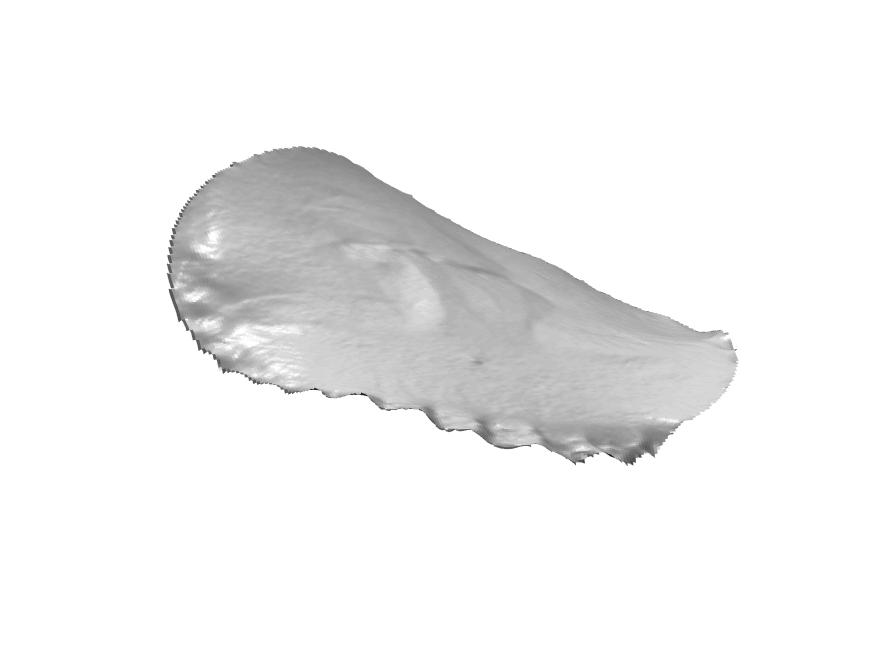
\includegraphics[width=5.5cm]{Buddha2}
		\caption{Top}
	\end{subfigure}%
	\begin{subfigure}{.33\textwidth}
		\centering
		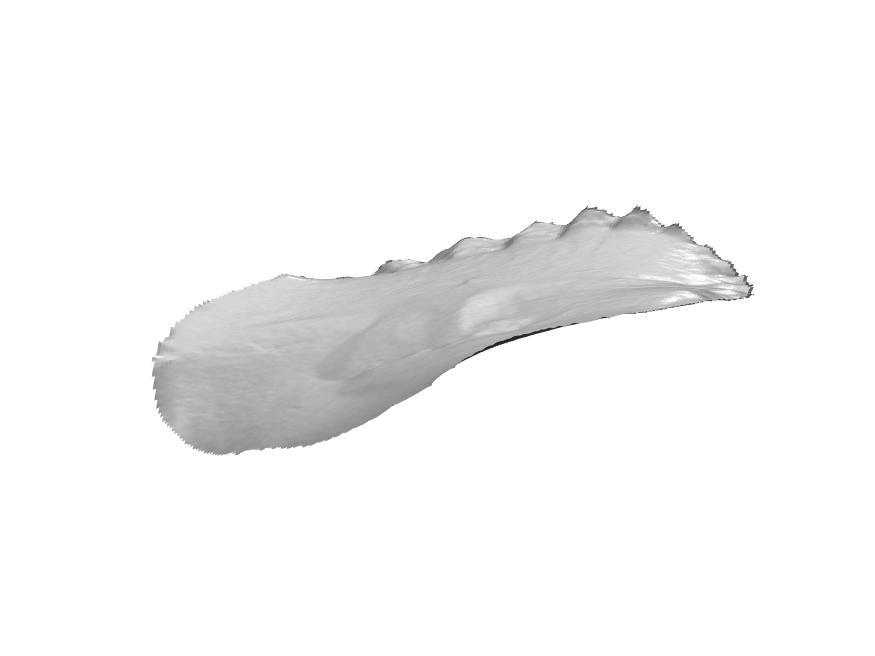
\includegraphics[width=5cm]{Buddha3}
		\caption{Bottom}
	\end{subfigure}
	\caption{The Buddha depth map from different view points}
	\label{fig:BuddahDepth}
\end{figure}

\begin{figure}[H]
	\centering
	\begin{subfigure}{.5\textwidth}
		\centering
		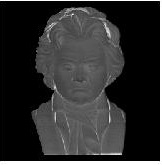
\includegraphics[height=6cm]{BeethovenAlbedo}
		\caption{The albedo for Beethoven}
	\end{subfigure}%
	\begin{subfigure}{.5\textwidth}
		\centering
		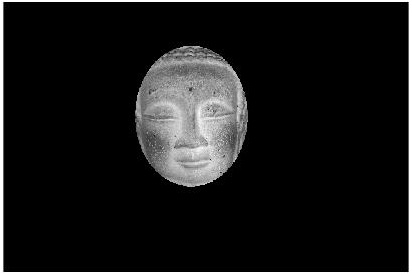
\includegraphics[height=6cm]{BuddhaAlbedo}
		\caption{The albedo for Buddha}
	\end{subfigure}
	\caption{The calculated albedo for Beethoven and Buddha}
	\label{fig:albedo}
\end{figure}

\end{document}